\documentclass[a4paper]{report}

\usepackage[top=2cm, bottom=2cm, left=2cm, right=2cm]{geometry}
\usepackage[utf8]{inputenc}
\usepackage[french]{babel}
\usepackage{textcomp}
\usepackage{layout}
\usepackage{color}
\usepackage{tcolorbox}
\usepackage{pxfonts}
\usepackage{indentfirst}
\usepackage{hyperref}
\usepackage{xifthen}% provides \isempty test
\usepackage{todonotes}

%
% Config
%
\setcounter{secnumdepth}{4}
\setcounter{tocdepth}{4}

% hyperref
\hypersetup{
    colorlinks=true,
    linkcolor=black,
    urlcolor=blue
}

\urlstyle{same}

% tcolorox
\tcbuselibrary{listings,skins}

\lstdefinestyle{bash}{
  language=bash,
  commentstyle=\color{red},
  basicstyle=\ttfamily,
  keywordstyle=\color{green!55!blue}\bfseries,
  morekeywords={docker, sudo, su, ssh, module, load, mysql, JBPMmicroscope, mysqlagcdb, ln},
  breaklines=true,
  frame=trBL
}

\lstdefinestyle{SQL}{
  language=SQL,
  breaklines=true,
  frame=trBL
}

\newtcolorbox{mycolorbox}
{
  colback=red!5!white,
  colframe=red!75!black,
  sharp corners=uphill,
  fonttitle=\bfseries,
  title=\textsc{Attention}
}

% Commands
\newcommand{\filename}[1]{\textbf{#1}}
\newcommand{\script}[1]{\textbf{#1}}
\newcommand{\module}[2][]{
    \texttt{#2\ifthenelse{\isempty{#1}}%
        {}% if version is empty
        {/#1}% if version is not empty}}
    }
}
\newcommand{\micWEBdeploy}{\module{micWEBdeploy}}
\newcommand{\micWEBdeployVer}{\module[0-MicroCloud-1.0]{micWEBdeploy}}
\newcommand{\cloudInstance}[1]{\textbf{#1}}
\newcommand{\component}[1]{\textbf{#1}}

\title{MicroCloud}
\author{Laura Burlot \and Mathieu Dubois}
\date{\today}

\begin{document}

\maketitle
\sloppy
\newpage

\tableofcontents
\newpage

\listoftodos

\begin{abstract}
Ce document présente le projet MicroCloud.
Il vise en particulier à donner une vue d'ensemble des choix effectués
et de leur implémentation ainsi qu'à fournir un guide utilisateur.

\begin{mycolorbox}
    La technologie SlipStream n'est plus maintenue et est obsolète.
    Le service Nuvla a pris fin le 15 mai 2020 peu de temps après la fin du projet.
    Le rapport présente ce qui fonctionnait à la fin du mois d'avril 2020.
    Ainsi, une partie des informations de ce rapport (liens vers les composants Nuvla) n'est plus pertinente.\\
    L'IFB a déployé sa propre instance de SlipStream mais nous n'avons pas accès à un équivalent de Nuvla pour modifier les composants.
    De plus, à l'heure actuelle, le déploiement de l'application MicroCloud depuis le catalogue RAINBio ne fonctionne pas.\\
    L'IFB est en train d'étudier de nouvelles solutions comme la solution Terraform Cloud en remplacement (pas de délais annoncés pour le moment, dépendra des ressources humaines disponibles). Quelle que soit la solution retenue, le mode de fonctionnement basé sur des scripts dans un dépôt git restera le même.
\end{mycolorbox}
\end{abstract}

\part{Vue d'ensemble du projet}

\section{Introduction}

Ce document présente le projet MicroCloud.
Il vise en particulier à donner une vue d'ensemble des choix effectués
et de leur implémentation ainsi qu'à fournir un guide utilisateur.

\begin{mycolorbox}
	La technologie SlipStream n'est plus maintenue et est obsolète.
	Le service Nuvla a pris fin le 15 mai 2020 peu de temps après la fin du projet.
	Le rapport présente ce qui fonctionnait à la fin du mois d'avril 2020.
	Ainsi, une partie des informations de ce rapport (liens vers les composants Nuvla) n'est plus pertinente.\\
	L'IFB a déployé sa propre instance de SlipStream mais nous n'avons pas accès à un équivalent de Nuvla pour modifier les composants.
	De plus, à l'heure actuelle, le déploiement de l'application MicroCloud depuis le catalogie RAINBio ne fonctionne pas.\\
	L'IFB est en train d'étudier de nouvelles solutions comme la solution Terraform Cloud en remplacement (pas de délais annoncés pour le moment, dépendra des ressources humaines disponibles). Quelle que soit la solution retenue, le mode de fonctionnement basé sur des scripts dans un dépôt git restera le même.
\end{mycolorbox}

\subsection{Objectifs du projet MicroCloud}

L'objectif du projet est de pouvoir déployer une instance de MicroScope dans le cloud.

\subsection{Documentation et code du projet}

\begin{itemize}
	\item Projet GitHub biosphere-microcloud : \url{https://github.com/IFB-ElixirFr/biosphere-microcloud}
	\item Projet GitHub biosphere-commons : \url{https://github.com/IFB-ElixirFr/biosphere-commons}
	\item Application MicroCloud : \url{https://nuv.la/module/ifb/devzone/MicroCloud/}
	\item Catalogue RAINBio : \url{https://biosphere.france-bioinformatique.fr/catalogue/}
	\item Appliance MicroCloud : \url{https://biosphere.france-bioinformatique.fr/catalogue/appliance/150/}
	\item Redmine du projet : \url{https://intranet.genoscope.cns.fr/agc/redmine/projects/microcloud} 
	\item Documents sur le cloud IFB: voir le wiki du projet Redmine et dans \path{/env/cns/proj/bureautique/agc/Formations_Suivies/20180619-Formation-Cloud-IFB}
\end{itemize}

\subsection{Contacts importants}

\begin{itemize}
	\item Contact général: Mathieu Dubois (\href{mailto:mdubois@genoscope.cns.fr}{mdubois@genoscope.cns.fr}), Genoscope
	\item Dépôt \href{https://github.com/IFB-ElixirFr/biosphere-commons}{biosphere-commons}: Christophe Blanchet (\href{mailto:Christophe.BLANCHET@france-bioinformatique.fr}{Christophe.BLANCHET@france-bioinformatique.fr}), PRABI UCBL1 Lyon
	\item Cloud prabi-girofle et problèmes d'accès à la VM permanente: Stéphane Delmotte (\href{mailto:Stéphane.Delmotte@univ-lyon1.fr}{Stéphane.Delmotte@univ-lyon1.fr}), PRABI UCBL1 Lyon
	\item Installation du serveur mysql dans la VM permanente: Sylvain Bonneval (\href{mailto:bonneval@genoscope.cns.fr}{bonneval@genoscope.cns.fr}), Genoscope
	\item Ouverture des ports pour accéder à la VM permanente: Guy Perrière (\href{mailto:guy.perriere@univ-lyon1.fr}{guy.perriere@univ-lyon1.fr}), Directeur du PRABI UCBL1 Lyon
\end{itemize}


\chapter{Bilan et perspectives}

\section{Bilan}

\subsection{Un prototype fonctionnel}

Le projet a permis de déployer une instance de MicroScope sur le cloud IFB
comprenant la partie web, les BD et les WF de calcul.
Le prototype permet faire tourner un WF simple (DIRECTON).

Pour cela, nous avons réalisé un script d'installation de MicroScope.
Ainsi, nous avons pu mieux comprendre les interactions entre les composants.
Ceci a été en particulier utile pour le composant \component{jbpmmicroscope} dont l'installation et la configuration
se sont avérées très délicates.

\todo[inline]{Il faut sans doute rajouter des choses dans cette partie.}

\subsection{Prise en main de BioMAJ et améliorations}

Un des objectifs du projet était d'utiliser \href{https://biomaj.genouest.org/}{BioMAJ}
pour la mise à jour des banques dans le cloud.

Le projet nous a permis de prendre en main le logiciel ce qui est intéressant car
il est utilisé dans le projet PanGBank.
De plus, il envisagé pour la copie des banques au Genoscope en remplaçant de Cabri.

Au cours du projet, nous avons ajouté plusieurs fonctionnalités à BioMAJ:
\begin{itemize}
	\item Utilisation des hardlinks lors de la mise à jour d'une banque (ce qui est plus rapide et consomme moins de place).
	\item Ajout d'options SSL (pour configurer l'accès aux ressources FTPS/HTTPS).
	\item Refactoring des downloaders (nettoyage du code).
	\item Possibilité de configurer le comportement en cas d'échec du téléchargement (combien de temps attendre et combien de fois ré-essayer).
\end{itemize}

Ce travail bénéficie à toute la communauté.

\subsection{Identification de limites dans l'architecture de MicroScope}

\todo[inline]{Fonctionnement sans données, frontières entre composants peu claires, dépendances.}

\subsection{Identification de limites de l'architecture cloud}

Le projet a aussi permis d'identifier un certains nombre de limites des architectures cloud.
Ces limites concernent principalement le stockage.

En effet, on ne veut pas reconstituer les banques pour chaque instance de MicroCloud.
Pour cela, nous  avons déployé une VM permanente dans le cloud \cloudInstance{ifb-prabi-girofle}
qui héberge les BD MySQL représentant les banques.\todo{Lien vers une section qui donne les détails techniques.}
Cependant, nous n'avons pas suffisamment de place pour télécharger toutes les banques de MicroScope sur la VM permanente.
À l'heure actuelle, seule la banque UNIPROTKBDB est disponible.

Une solution partielle est le stockage permanent et partagé mis en place par l'IFB
qui est utilisé pour mettre à disposition les banques sur toutes les VM (ces banques sont mises à jour avec BioMAJ).
On pourrait alors utiliser les WF de mise à jour des banques de MicroScope.
Cependant ceci n'est pas encore disponible sur \cloudInstance{ifb-prabi-girofle} (sur lequel tourne la VM permanente).

\section{Limites}

Outre les limites évoquées plus haut, le prototype a plusieurs limites:
\begin{itemize}
	\item La version de MicroScope n'est pas fixée: les scripts d'installation incluent la dernière version disponible sur les serveurs du Genoscope.
	\item À cause des ces limites, MicroCloud ne tourne que le cloud \cloudInstance{ifb-prabi-girofle}.
	\item Du fait que les banques sont mises-à-jour manuellement sur la VM permanente, on peut avoir un décalage entre la version de MicroScope déployée dans le cloud
	et la version des banques sur la VM.
\end{itemize}

\section{Améliorations}

Les principales améliorations au prototype sont:
\begin{itemize}
	\item Résoudre le problèmes des banques. Ceci passe sans doute par l'améliorations de l'infrastructure de Biosphere.
	\item Améliorer l'installation des dépendances pour les WF.
\end{itemize}

D'un point de vue technique, les améliorations sont:
\begin{itemize}
    \item Améliorations du côté de biosphère-commons (option -e).
    \item Certains scripts sont sourcés avec une option (ce qui est valide en bash mais n'est pas portable).
    \item Paralléliser les scripts pour diminuer le temps de déploiement (en particulier pouvoir faire le maximum de choses avant d'attendre les signaux des autres composants).
    \item le module \module{micPrestation} (utilisé pour insérer des organismes sans faire de prestation) ne fonctionne pas suite aux modifications du schéma de TAXONOMYDB.
\end{itemize}

Le code de déploiement des VM contient une liste d'améliorations (voir le fichier \filename{README.md} dans le répertoire de chaque composant sur le dépôt \href{https://github.com/IFB-ElixirFr/biosphere-commons}{GitHub biosphere-commons}).


\part{Guide d'utilisation}

\chapter{Déployer une instance MicroCloud et l'utiliser} \label{chap:deploiement}

Ce chapitre décrit l'utilisation de MicroCloud d'un point de vue utilisateur.
Le lecteur est invité à lire la documentation sur le cloud IFB
(voir \href{https://intranet.genoscope.cns.fr/agc/redmine/documents/86}{les documents de la formation IFB},
\href{https://intranet.genoscope.cns.fr/agc/redmine/issues/6010}{la demande liée}
et la page \href{https://intranet.genoscope.cns.fr/agc/redmine/projects/microcloud/wiki/Principes_de_fonctionnement_du_cloud_IFB}{[[Principes de fonctionnement du cloud IFB]]}
dans le projet Redmine).

\section{Déployer l'appliance MicroCloud}

L'appliance MicroCloud est disponible dans le catalogue RAINBio \url{https://biosphere.france-bioinformatique.fr/catalogue/appliance/150/}.
Pour déployer l'appliance, cliquer sur \textbf{Lancer}.
En utilisant \textbf{Déploiement avancé}, on peut choisir le nombre de nœuds de calculs.

Les déploiements se font sur le cloud \cloudInstance{ifb-prabi-girofle} sur lequel est installé la \hyperref[VM permanente]{VM permanente}.
Un déploiement prend environ 40 minutes.

\bigskip

Il y a 2 points d'entrée du déploiement:
\begin{enumerate}
	\item \emph{L'interface web:} L'URL de la plateforme est: \nolinkurl{https://${IP_frontend}/home/index.php} où \nolinkurl{${IP_frontend}}
	      est l'IP de la machine frontend.
	      Cette URL est reporté dans l'interface RAINBio.
	\item \emph{La machine frontale du cluster:} On peut aussi se connecter en SSH à la machine frontale du cluster
	      dont l'IP est aussi reportée dans l'interface de RAINBio.
	      Cette machine comprend les modules nécessaire au travail avec une instance (\module{micGenome}, \module{micJBPMwrapper}, etc.)
	      et \component{jbpmmicroscope} pour déployer les WF.
	      La plupart des chemins sont identique
\end{enumerate}
L'instance fournie contient les données de \textit{Acinetobacter baylyi} ADP1.
Cependant, l'instance fournie ne contient pas d'utilisateur
et aucun WF n'est configuré sur l'instance.
De plus, les logiciels métier des WF ne sont pas installés.

\section{Créer un nouvel utilisateur admin}

Une fois l'instance déployée, il faut créer un utilisateur admin.

Pour cela, il faut se connecter en ssh à la frontale puis exécuter le script \script{create\_user.sh}:
\begin{lstlisting}[style=Bash]
	ssh centos@${IP_master}
	cd \path{/var/tmp/slipstream/biosphere-microcloud/master}
	./create_user.sh LOGIN EMAIL admin
\end{lstlisting}
Le script demande le mot de passe à utiliser et crée l'utilisateur

\section{Insérer un nouvel organisme (partie Syntactic)}

La première étape est d'ajouter les données de taxonomie pour ce nouvel organisme.
Pour cela, il faut mettre à jour la base TAXONOMYDB de la VM permanente :
\begin{itemize}
	\item en copiant les données de prod de TAXONOMYDB et pkgdb.O\_Taxonomy pour cet organisme
	\item ou en déployant les WF TAXONOMYDB et TAXONOMY
\end{itemize}
\bigskip

Pour insérer un nouvel organisme, on utilise le module \module{micPrestation}.
La procédure à suivre est la suivante :
\begin{enumerate}
	\item Télécharger un fasta et décompresser l'archive.
	\item Remplir le fichier Template\_Prestation.csv qui trouve dans le répertoire \path{/env/cns/proj/agc/module/products/micsyntactic/unix-noarch/lib}.
	\item Lancer la création de la prestation:
          \begin{lstlisting}[style=bash]
            $ prestaBatch.py --csv Template_Prestation.csv -sd ${working_dir} -A ${Annotator_name} -T genome
          \end{lstlisting}
          Il y a un exemple de fichier Template\_Prestation.csv dans le dossier prestation : \path{/env/cns/wwwext/html/agc/ftp/MicroCloud/prestation}.
    \item Accepter la prestation:
          \begin{itemize}
          	\item Depuis le web (avec l'utilisateur admin crée à la section précédente).
          	\item Pour valider la prestation sans passer par le web faire :
          	      \begin{lstlisting}[style=SQL]
          	      	USE PRESTATIONDB;
          	      	SELECT * FROM Prestation;
          	      	UPDATE Prestation SET PS_status='accepted' WHERE PS_status='inprogress';
    	          \end{lstlisting}
           \end{itemize} 
\end{enumerate}

Puis, pour insérer la nouvelle séquence en base, utiliser le module \module{micGenome}:
\begin{lstlisting}[style=bash]
  $ loadGenomeNS.sh -p ${PS_id} -o ${O_id}
\end{lstlisting}

\begin{mycolorbox}
    Les données des banques nécessaires pour le script \textbf{loadGenomeNS.sh} ne sont pas stockées dans la VM permanente actuellement (données des banques gérées par CABRI).
    Cette étape ne fonctionne donc pas.
\end{mycolorbox}
\todo[inline]{Quelles banques ? TAXONOMY ? Mettre à jour la référence dans les limites}

\section{Déployer un WF}

Les workflows sont déployés sur la VM master.
À ce jour nous n'avons pu tester que le workflow DIRECTON.
Les sources du moteur de workflow (\component{jbpmmicroscope}) sont dans le répertoire \path{/env/cns/proj/agc/tools/COMMON/JBPMmicroscope/jbpmmicroscope}.
Le répertoire de travail Tomcat est le suivant : \path{/env/cns/proj/agc/tools/COMMON/JBPMmicroscope/tomcat}.
Les modules sont localisés dans le répertoire : \path{/env/cns/proj/agc/module/products}
\newline

\begin{mycolorbox}
	Si les données ont été copiées depuis la prod et insérées telles quelles (sans \module{micPrestation}), il faut, dans la table pkgdb.Sequence, vérifier que le status des S\_id existants soit 'inFunctional' et non 'inProduction' pour que les WF prennent bien en compte les nouveaux S\_id.
\end{mycolorbox}

\begin{lstlisting}[style=SQL]
USE pkgdb;
UPDATE Sequence SET S_status='inFunctional' WHERE S_status='inProduction';
\end{lstlisting}

\subsection{Déployer le WF DIRECTON}
Les modules requis pour le bon déploiement de ce workflow sont les suivants : \textbf{bagsub-2.4.3}, \textbf{AGCScriptToolMic-2.0}, \textbf{micGenome-7.0.0}, \textbf{micJBPMwrapper-3.10.8} et \textbf{micPrestation-2.0} et \textbf{micDirecton-1.0}.

\begin{lstlisting}[style=bash]
#### Deploy DIRECTON WF ####
$ cd /env/cns/proj/agc/tools/COMMON/JBPMmicroscope/tomcat/

# Deploy WF
$ JBPMmicroscope deployProcess -dirXMLSrc ../jbpmmicroscope/src/main/process-definitions/jpdl/BagSub/ -defNames DIRECTON

# Deploy and start CRON
$ JBPMmicroscope deployProcess -dirXMLSrc ../jbpmmicroscope/src/main/process-definitions/jpdl -defNames CRON_DIRECTON
JBPMmicroscope startCron -names CRON_DIRECTON

# Check CRON and WF status
$ JBPMmicroscope showProcessDefinitions

# Force run
$ JBPMmicroscope signalCron -names CRON_DIRECTON -signal forceRun; JBPMmicroscope signalProcess -pid 1

$ JBPMmicroscope showProcessInstances

# Take a look at running processes
$ tomcat_logs

# relaunch WF if status is sendmail
$ JBPMmicroscope relaunchAnalysis -pidCron 1 -pidWF 2 -signal forceRun

# Check tables pkgdb.Workflow_Jobs, pkgdb.Directon and pkgdb.GO_Directon_CPD
$ mysqlagcdb
\end{lstlisting}


\chapter{Mettre à jour des composants pour MicroCloud} \label{chap:creer_nouvelle_version}

\begin{mycolorbox}
	METTRE ICI LES COMMANDES POUR CRÉER DES RELEASES, COPIER DES BASES, etc.
\end{mycolorbox}

Ce chapitre présente les commandes utilisées pour créer une nouvelle version
du code et des données qui seront déployées sur le cloud.
Ces opérations utilisent le module \micWEBdeployVer
et doivent être effectuées au Genoscope.
Par convention le répertoire d'export des archives et autres fichiers sur etna0: \path{/env/cns/wwwext/html/agc/ftp/MicroCloud/}.
\bigskip

Pour charger le module \micWEBdeployVer:
\begin{lstlisting}[style=bash]
$ module load micWEBdeploy/0-MicroCloud-1.0
\end{lstlisting}

\section{Créer une nouvelle release du code web}

Pour créer une nouvelle version du code du web et des bases de données:
\begin{lstlisting}[style=bash]
$ MICVERSION=3.14.0
$ microscopeRelease.py --version ${MICVERSION} --output /env/cns/wwwext/html/agc/ftp/MicroCloud/microcloud-${MICVERSION}.tar.gz
\end{lstlisting}

Ensuite, mettre à jour le lien symbolique pour qu'il pointe vers la nouvelle archive :
\begin{lstlisting}[style=bash]
$ cd /env/cns/wwwext/html/agc/ftp/MicroCloud
$ ln -s microcloud-${MICVERSION}.tar.gz microcloud-latest.tar.gz
\end{lstlisting}

\section{Copier les données d'un organisme}

Permet de copier les données de l'organisme \textit{Acinetobacter baylyi} (O\_id=31).

\begin{mycolorbox}
	Pour le moment seules les données concernant l'O\_id 31 peuvent être récupérées avec le script microscopeCopyOid.py car certains organismes ont besoin de tables spécifiques de la base GO\_SPE (typiquement la table acineto\_KO pour Acinetobacter baylyi).
\end{mycolorbox}

\begin{lstlisting}[style=bash]
$ Oid=31
$ microscopeCopyOid.py --oid ${Oid} --output /env/cns/wwwext/html/agc/ftp/MicroCloud/microscope_${Oid}.tar.gz
\end{lstlisting}

Ensuite, mettre à jour le lien symbolique pour qu'il pointe vers la nouvelle archive :
\begin{lstlisting}[style=bash]
$ Oid=31
$ cd /env/cns/wwwext/html/agc/ftp/MicroCloud
$ ln -s microscope_${Oid}.tar.gz microscope_${Oid}-latest.tar.gz
\end{lstlisting}

\section{Mettre à jour jbpmmicroscope}

Dans cette section JBPMmicroscope peut faire référence à la base de données JBPMmicroscope ou bien à la commande JBPMmicroscope qui permet le déploiement des WF.
\newline

Il faut générer les fichiers suivants :
\begin{itemize}
	\item \script{jbpmmicroscope.jar}
	\item \script{SystemActorsLauncher.jar}
	\item \script{jbpmmicroscope-server.war}
\end{itemize}
\bigskip

Puis mettre à jour le fichier \path{~/.m2/genosphere-settings.xml} :
\begin{itemize}
	\item  Mettre à jour le local path
	\item Supprimer/modifier le login et le mot de passe
\end{itemize}

Pour créer les .jar dans le répertoire \path{jbpmmicroscope-client/target/} faire :

\begin{lstlisting}[style=bash]
$ mvn -Pconfig-microcloud -s ~/.m2/genosphere-settings.xml clean install
\end{lstlisting}
\bigskip

Il faut ajouter les sources (pour le déploiement des WF) et le script JBPMmicroscope
\begin{lstlisting}[style=bash]
$ jar uf jbpmmicroscope-client/target/jbpmmicroscope.jar -C ./ src/
$ jar uf jbpmmicroscope-client/target/jbpmmicroscope.jar -C ./ JBPMmicroscope
\end{lstlisting}
\bigskip

Pour créer l'archive \path{jbpmmicroscope-server.war} dans le répertoire \path{jbpmmicroscope-server/target/} :
\begin{lstlisting}[style=bash]
$ mvn -Pconfig-microcloud -s ~/.m2/genosphere-settings.xml package
\end{lstlisting}
\bigskip

Copier le .war et les .jar sur etna0 dans le répertoire \path{/env/cns/wwwext/html/agc/ftp/MicroCloud/}
La VM master importe ces fichiers à l’aide des liens symboliques.
\newline

Le schéma de la base JBPMmicroscope est créé automatiquement par hibernate (\script{hibernate.cfg.xml} voir le paramètre \textbf{hbm2ddl.auto}) lors de la première exécution d'une commande JBPMmicroscope.
\newline

Les identifiants de connexion à la base JBPMmicroscope (hibernate) sont les suivants :
login: \textbf{jbpm} et password: \textbf{jbpm}. Ces identifiants peuvent être modifiés dans le composant master, ils correspondent aux paramètres \textbf{jbpm\_user} et \textbf{jbpm\_password} (penser à mettre à jour le fichier \path{hibernate.cfg.xml}, régénérer les .jar et le .war et les copier dans \path{/env/cns/wwwext/html/agc/ftp/MicroCloud}).
\newline

jbpmmicroscope nécessite un serveur Tomcat pour fonctionner. Tomcat 9 est installé dans le composant master : \path{/env/cns/proj/agc/tools/COMMON/JBPMmicroscope/tomcat}. Les identifiants tomcat sont les suivants : login: \textbf{tomcat} et password: \textbf{tomcat}.
Ces identifiants peuvent être modifiés dans le composant master : paramètres \textbf{tomcat\_user} et \textbf{tomcat\_password}.

\section{Mettre à jour la VM permanente}
\todo{compléter cette partie}
Pour cela s'inspirer du script \script{microscopeCreateDBschemas.py}, copier les fichiers ainsi générés sur la VM permanente et les insérer en base.

\section{Mettre à jour les scripts côtés serveur}

Mettre à jour (si besoin) les scripts \script{import\_Oid.sh} et \script{install\_microscope.sh}.


\part{Détails techniques}

\chapter{Architecture}

Dans ce chapitre, on ne fait pas toujours la distinction entre un composant (au sens de composant SlipStream)
et une VM (qui est un composant déployé).
Il faut toutefois rappeler qu'un composant peut être déployé plusieurs fois.

De la même manière, nous utilisons le mot \og{} composant \fg{} pour parler d'un composant SlipStream
et d'un composant (logiciel) de MicroScope.
Le contexte devrait permettre d'éviter toute ambiguïté.

\section{Vue d'ensemble}

La vue d'ensemble de l'architecture est présentée dans la~\autoref{fig:architecture}.
Il y 5 composants Nuvla et
1 VM permanente déployée sur le cloud \cloudInstance{ifb-prabi-girofle}.

\begin{figure}[htp]
    \centering
    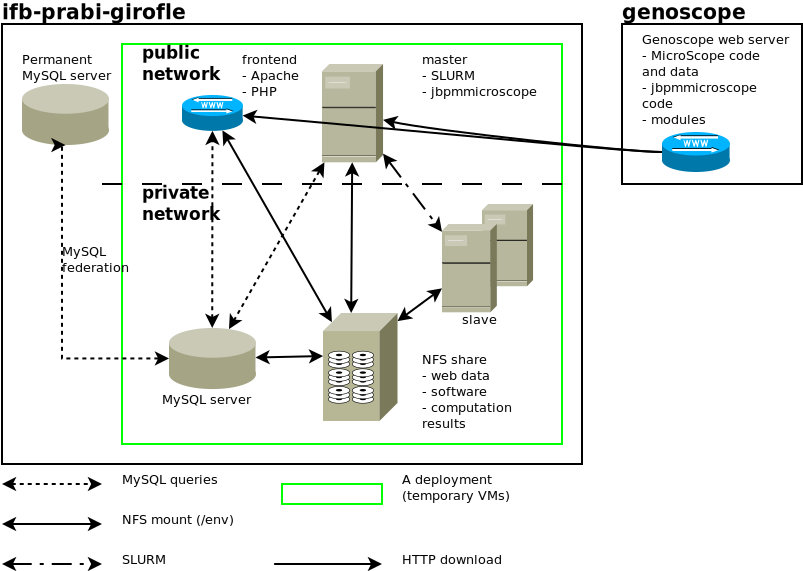
\includegraphics[width=\linewidth]{../Logical_Architecture}
    \caption{Schéma de l'architecture de MicroCloud.}
    \label{fig:architecture}
\end{figure}

Un des buts est de mimer ce qui est fait au Genoscope
c'est-à-dire que:
\begin{enumerate}
    \item Les différents composants (serveur web, serveur de BD, etc.) tournent sur des machines séparées.
    \item Les calculs tournent sur des machines séparées: l'architecture contient donc un cluster (basé sur SLURM).
\end{enumerate}
Une des seules différences est que le serveur \component{jbpmmicroscope} tourne
sur la machine frontale du cluster.

Lors du déploiement, les VM téléchargent des fichiers (code et données) depuis le serveur web du Genoscope.
Ces fichiers sont crées par le module \micWEBdeployVer{} (voir~\autoref{chap:micwebdeploy}).
Le gros du travail du travail est fait dans les scripts de la phase Deployment (script \script{04\_Deployment.sh} de chaque composant SlipStream).
Ceci a été fait pour simplifier les scripts d'installation et ne pas fixer les versions de MicroScope à ces étapes.

Il y a 2 serveurs de bases de données dans MicroCloud\todo{Renvoyer à section choix techniques.}:
\begin{itemize}
    \item Un serveur MySQL installé via Docker dans la VM MySQL.
    \item Un serveur MySQL sur la VM permanente.
\end{itemize}

\section {Installation et déploiement des VM}

Le code des composants Nuvla est dans le dépôt \project{biosphere-microcloud}.
Il y a un dossier par composant et un fichier \filename{README.md} dans chaque dossier qui explique des détails.
Les principes du déploiement sont décrits sur le wiki du projet (voir la page
\href{https://intranet.genoscope.cns.fr/agc/redmine/projects/microcloud/wiki/Principes_de_fonctionnement_du_cloud_IFB}
{[[Principes de fonctionnement du cloud IFB]]}
en particulier la section
\href{https://intranet.genoscope.cns.fr/agc/redmine/projects/microcloud/wiki/Principes_de_fonctionnement_du_cloud_IFB#Utilisation-de-deacutepocircts-git-pour-le-code}
{[[Utilisation de dépôts git pour le code]]}
).

Les sections suivantes présentent quelques détails sur les VM:
\begin{itemize}
    \item \SScomponent{frontend} voir section \ref{frontend}
    \item \SScomponent{mysql} voir section \ref{mysql}
    \item VM permanente voir section \ref{VMpermanente}
    \item \SScomponent{master} et \SScomponent{slave} voir section \ref{master&slave}
    \item \SScomponent{nfsserver} voir section \ref{nfsserver}
\end{itemize}
Comme expliqué, le code de chaque composant est dans un dossier éponyme dans le dépôt biosphere-microcloud.
Dans les sections sus-citées, le nom des scripts est relatif à ce dossier (sauf mention contraire).

\subsection {Composant \SScomponent{frontend}}\label{frontend}

La composant \SScomponent{frontend} permet de déployer la partie web de la plateforme MicroScope.
L'image de base est une image CentOS 7.

\paragraph*{Configuration}

Le script \script{04\_Deployment.sh} réalise un certain nombre d'opérations avant l'installation de MicroScope:
\begin{itemize}
    \item Configuration de \component{Apache} (génération d'un certificat SSL)
          et \component{PHP} (variables \variable{memory\_limit}, \variable{max\_execution\_time},  \variable{max\_input\_time})
          nécessaires pour MicroScope.
    \item Configuration d'un alias du composant \SScomponent{mysql} sous le nom \hostname{mysqlagcdb.genoscope.cns.fr}
          (ceci a été fait pour ne pas avoir à modifier la configuration de MicroScope).
    \item Configuration de \component{phpMyAdmin}.
    \item Montage du répertoire partagé.
\end{itemize}

\begin{mycolorbox}
    La VM \SScomponent{frontend} utilise un client mariaDB (et non pas MySQL du fait de conflits existants entre le dépôt remi-php71 installé et le dépôt IUS qui fournit le client MySQL).
\end{mycolorbox}

\paragraph*{Installation de MicroScope}

Le script \script{install\_microscope.sh} réalise l'installation de MicroScope:
\begin{itemize}
    \item Création de l'utilisateur MySQL \user{agc} (avec le mot de passe habituel).
    \item Création des bases de données nécessaires à l'instance et copie des données minimales.
          Les tables nécessaires à l'installation de MicroScope (hors bases des banques qui sont dans la VM permanente)
          sont listées dans la page wiki           \href{https://intranet.genoscope.cns.fr/agc/redmine/projects/microcloud/wiki/Tables_necessaires_a_installation}{[[Tables nécessaires à l'installation]]}.
    \item Copie du code web dans le répertoire \variable{DOCUMENT\_ROOT} de la VM (\path{/var/www/html/})
          et des scripts dans \path{/var/www/binphp/} (variable \variable{BIN} dans la configuration de MicroScope).
\end{itemize}

\paragraph*{Import des données de l'organisme \theOrg{}}

Les données de \theOid{} sont copiées avec le script \script{import\_Oid.sh}.

\begin{mycolorbox}
    Si lors de la connexion au serveur web le message d'erreur \textbf{256} s'affiche, cela signifie qu'il n'y a pas d'organisme en base.
    De ce fait, la plupart des onglets ainsi que le formulaire d'authentification sont inaccessibles.
    Ceci ne doit pas arriver si le déploiement se passe bien car on on copie les données d'un organisme.
\end{mycolorbox}

\paragraph*{Création des liens FEDERATED}

Les liens FEDERATED vers la VM permanente (qui permettent d'accéder aux base représentant les banques) sont crées
dans le script \script{create\_federated\_links.sh}.
Le script crée automatique un lien avec toutes les BD présentes sur la VM permanente sauf les BD système (\DB{mysql}, \DB{information\_schema}, \DB{performance\_schema}, \DB{sys})
et celles liées à \component{phpMyAdmin}.

\subsection {Composant \SScomponent{mysql}}\label{mysql}

Le composant \SScomponent{mysql} est le serveur de base de données de l'instance.
L'image de base est une image CentOS 7.

Comme cette VM se trouve sur le réseau privé, il faut passer par la VM frontend pour se connecter à la VM mysql:
\begin{lstlisting}[style=bash]
ssh -A centos@${IP_mysql} -J centos@${IP_frontend}
\end{lstlisting}

\paragraph*{Installation de MySQL}

Le serveur MySQL est installé via Docker.
Si le serveur ne répond pas, il faut aller voir si le docker n'a pas planté (cela arrive pour des requêtes SQL trop gourmandes en RAM).
Pour relancer le docker :
\begin{lstlisting}[style=bash]
sudo su
docker ps -a
docker start ${ID_container}
\end{lstlisting}

\paragraph*{Installation des fonctions UDF de MicroScope}

Les fonctions UDF nécessaires à MicroScope (\component{lib\_mysqludf\_sequtils})
sont téléchargées depuis le Genoscope et
sont installées dans le docker.

\begin{mycolorbox}
    Contrairement à la plupart des autres composants, la version des fonctions UDF utilisée
    est fixée dans les scripts (\micUDFVersion) et n'est pas gérée par \micWEBdeployVer{} (voir~\autoref{chap:micwebdeploy}).
    Ceci est lié au fait que c'est le composant qui a été développé en premier
    et que \component{lib\_mysqludf\_sequtils} évolue peu.
\end{mycolorbox}

\subsection {VM permanente}\label{VMpermanente}

La procédure d'installation est dans le fichier \textbf{Installation.md} du répertoire \textbf{/root}. La VM permanente sert au stockage des données des banques. Nous avons utilisé \textbf{rsync} pour l'import des données dans le serveur MySQL.

Logiciels installés : serveur MySQL, rsync, phpMyAdmin (installé mais non configuré).

Pour se connecter :
\begin{lstlisting}[style=bash]
ssh root@134.214.33.214
\end{lstlisting}

\paragraph*{Création des BD et copie des données}

Le serveur MySQL contient les schémas des banques et les données nécessaires pour les tests (nous avons testés les onglets \textbf{Genome Browser}, \textbf{Identical Gene Names}):
\begin{itemize}
    \item les schéma des bases \DB{ANTISMASHDB}, \DB{CARDDB}, \DB{COGDB}, \DB{EGGNOGDB}, \DB{ENZYMEDB}, \DB{ESSDB}, \DB{FIGFAMDB}, \DB{INTERPRODATADB},
          \DB{KEGGDB}, \DB{RHEADB}, \DB{TAXONOMYDB}, \DB{TIGRFAMDB}, \DB{UNIFIREDB}, \DB{UNIPROTKBDB}, \DB{VIRULENCEDB}, \DB{microcyc}\footnote{Je pense cette base n'est pas nécessaire à l'heure actuelle (MD).}
          et \DB{DBWORKFLOW}.
    \item une partie des données de la base \DB{UNIPROTKBDB} pour les tests.
    \item les données de \DB{DBWORKFLOW}.
    \item les données de l'organisme \theOrg{} (taxon id \theTaxID{}) dans la base \DB{TAXONOMYDB}.
\end{itemize}

Le script \script{microscopeDBschema.py} du module MicroCloud a été utilisé pour créer les schémas.

Pour se connecter au serveur MySQL :
\begin{lstlisting}[style=bash]
mysql -p{MOT_DE_PASSE_SERVEUR_MYSQL_VM_PERMANENTE}
\end{lstlisting}

\subsection{Compoants \SScomponent{master} et \SScomponent{slave}} \label{master&slave}

\todo[inline]{Ajouter les notes sur jbpmmicroscope ici ? Notes sur conda et l'installation des modules ? Plutôt dans la partie choix techniques.}

Ces 2 composants permettent de créer un cluster basé sur SLURM sur lequel \component{jbpmmicroscope} soumet les jobs:
\SScomponent{master} est la frontale et \SScomponent{slave} est un nœud de calcul.
Le code SlipStream est basé sur les travaux de Jonathan Lorenzo et Bryan Brancotte:
\begin{itemize}
    \item Les composants \SScomponent{master} et \SScomponent{slave} ont été copiés depuis
    l'appliance \href{https://nuv.la/module/ifb/devzone/jlorenzo/cluster/Slurm_Cluster_ubuntu18}{\SScomponent{Slurm\_Cluster\_ubuntu18}}.
          L'image de base de ces composants est une image Ubuntu 18.04.
    \item Le code d'installation de ces composants a été copié depuis le dépôt \project{biosphere-commons}
          puis modifié pour les besoins de MicroCloud\todo{Préciser çà}.
\end{itemize}
Le composant \component{slave} peut être instancié plusieurs fois (2 par défaut).
Ceci est choisi lors du déploiement (voir~\autoref{chap:deploiement}).

\paragraph*{Généralités}

Les composants \SScomponent{master} et \SScomponent{slave} montent le dossier partagé \path{/env/} (voir~\autoref{nfsserver}).
Le composant \SScomponent{slave} est peu modifié par rapport aux scripts de J. Lorenzo et B. Brancotte.
En revanche, le composant \SScomponent{master} est plus complexe car
c'est sur lui qu'on installe \component{jbpmmicroscope} (et donc \component{Tomcat})
et les logiciels partagés entre la frontale et les nœuds de calcul.

\paragraph*{Installation de \component{jbpmmicroscope}}

\component{jbpmmicroscope} et le serveur d'application \href{http://mirrors.ircam.fr/pub/apache/tomcat/tomcat-9/v9.0.31/bin/apache-tomcat-9.0.31.tar.gz}{\component{Tomcat} version 9.0.31}
sont installés par \script{install\_jbpm.sh} à partir des fichiers téléchargés depuis le Genoscope.
Le script n'est pas très compliqué.

Pour accéder à Tomcat : http://\$IP\_master.

\paragraph*{Installation de \component{pegasus-mpi-cluster}}

\component{bagsub} s'appuie sur \component{pegasus-mpi-cluster}.
Nous avons installé (\href{https://github.com/pegasus-isi/pegasus/archive/4.9.2.zip}{\component{pegasus-mpi-cluster} version 4.9.2}).
Le code téléchargé ne compile pas à cause car la librairie \component{libnuma} n'est pas installée.
Comme celle-ci n'est pas nécessaire pour les architectures non-NUMA, nous modifions les fichiers \filename{Makefile}
pour supprimer la dépendance à \component{libnuma}.

\paragraph*{Installation des modules (dont \component{bagsub})}

Chaque workflow fait appel à différents modules qu'il faut installer au préalable sur la VM master.
Le script \script{import\_modules.sh} permet d'importer les archives des différents modules nécessaires au fonctionnement des workflows (WF DIRECTON principalement).

Le script \script{import\_modules.sh} fait quelques modifications du module \component{bagsub} afin qu'il puisse être utilisé dans l'environnement fourni par la VM \SScomponent{master}:
on supprime l'option ulimit qui ne fonctionne pas en \component{dash} (le shell sous Ubuntu 18.04)
et ajoute le paramètre MCA \variable{btl\_tcp\_if\_exclude} pour exclure les interfaces réseaux \hostname{docker0} et \hostname{lo} qui peuvent engendrer des conflits lors du lancement de jobs SLURM.


\subsection{Composant \SScomponent{nfsserver}} \label{nfsserver}

Le composant \SScomponent{nfsserver} a été créé en s'inspirant du travail de Stéphane Delmotte.
Il permet de fournir un dossier partagé entre les différentes VM.
L'image de base est une image CentOS 7.

Le répertoire \path{/var/nfsshare} du serveur NFS est monté dans le répertoire \path{/env}
des composants \SScomponent{frontend}, \SScomponent{backend}, \SScomponent{master} et \SScomponent{slave}.
Le répertoire \path{/env/} se veut similaire au répertoire de même nom sur le cluster \hostname{etna}.

Les fonctions permettant de monter le répertoire partagé sur les autres composants sont dans le fichier \script{lib.sh}
(qui est à la racine du dépôt \project{biosphere-microcloud} car il est utilisé par tous les composants).
Le code a été copié depuis le dépôt \project{biosphere-commons}.

% Faire un tableau récapitulatf ?

\chapter{Module \micWEBdeployVer} \label{chap:micwebdeploy}

Ce module contient les scripts utilisés côté Genoscope pour gérer les fichiers (logiciels et les données) nécessaires pour déployer MicroCloud (voir~\autoref{chap:creer_nouvelle_version}).
C'est une version de développement basée sur \module[1.0]{micWEBdeploy}.

Il est constitué des scripts suivants :
\begin{description}
    \item[\script{microscopeRelease.py}] : copie le code du web, compile le code JavaScript (avec \script{microscopeCompileJS.sh}), copie les schémas de certaines bases et les données minimales de certaines bases.
    \item[\script{microscopeCopyOid.py}] : permet de copier les données de l'organisme \theOrg{} (Oid=\theOid)
    \item[\script{createModulesTarball.py}]: créé les archives des modules à importer dans MicroCloud.
\end{description}

Comme expliqué, ce module est très lié aux scripts de déploiement des VM.

\section{\script{microscopeRelease.py}}

Les schémas copiés sont : pkgdb, REFSEQDB, GO\_Conf, GO\_RES, GO\_CPD, PUB\_CPD et PRESTATIONDB.

Les données copiées sont : pkgdb (tables : Maintenance, Country, Amiga\_Params,
Annotator pour A\_name='guest', Sequence\_Checkpoint\_Desc et Sid\_Config), GO\_RES (tables : ORGCLUST\_clustering\_param et ORGCLUST\_distance\_param.
) et GO\_Conf (prendre les données de toutes les tables). Voir page wiki : \url{https://intranet.genoscope.cns.fr/agc/redmine/projects/microcloud/wiki/Tables_necessaires_a_installation}


\section{\script{createModulesTarball.py}}

Créé les liens symboliques dans \path{/env/cns/wwwext/html/agc/ftp/MicroCloud}.
Créé le fichier \path{modules.txt} dans \path{/env/cns/wwwext/html/agc/ftp/MicroCloud}.
Puis, la VM master importe les modules listés dans modules.txt (voir \url{https://github.com/IFB-ElixirFr/biosphere-microcloud/blob/master/master/import_modules.sh}).

\begin{lstlisting}[style=bash]
createModulesTarball.py --modules_list bagsub-2.4.3 AGCScriptToolMic-2.0 micGenome-7.0.0 micJBPMwrapper-3.10.8 micPrestation-2.0 micDirecton-1.0
\end{lstlisting}

\section{\script{microscopeCopyOid.py}}

\begin{mycolorbox}
    Pour le moment seules les données concernant l'Oid \theOid{} peuvent être récupérées avec le script microscopeCopyOid.py car certains organismes ont besoin de tables spécifiques de la base GO\_SPE (typiquement la table acineto\_KO pour \theOrg{}).
\end{mycolorbox}

\begin{lstlisting}[style=bash]
Oid=(*\theOid{}*)
microscopeCopyOid.py --oid ${Oid} --output /env/cns/wwwext/html/agc/ftp/MicroCloud/microscope_${Oid}.tar.gz
\end{lstlisting}

\section{\script{microscopeCreateDBschemas.py}}
A permis de générer les .sql utilisés pour créer les schémas des bases de données dans la VM permanente.

\begin{lstlisting}[style=bash]
microscopeCreateDBschemas.py --output /env/cns/wwwext/html/agc/ftp/MicroCloud/DBschemas.tar.gz
\end{lstlisting}

\section{\script{taxonomyDBCopyTaxId.py}}
Permet de copier les données de la base TAXONOMYDB pour un tax\_id donné.

\begin{lstlisting}[style=bash]
taxonomyDBCopyTaxId.py --tax_id 202950 --output /env/cns/wwwext/html/agc/ftp/MicroCloud/taxonomyDBCopyTaxId.tar.gz
\end{lstlisting}

\section{Les scripts côté serveur}

Les scripts coté serveur importent et utilisent les fichiers générés par le module \micWEBdeployVer.

Les scripts concernant l'installation de MicroScope sont dans le dossier \textbf{frontend} \url{https://github.com/IFB-ElixirFr/biosphere-microcloud/blob/master/master} :
\begin{description}
    \item[\script{install\_microscope.sh}] Le frontend est basé sur Apache2, PHP7.1 et phpMyAdmin. L'installation est double : il faut d'abord configurer quelques bases (Apache2, PHP7.1 et phpMyAdmin) et monter le répertoire partagé après avoir configuré MicroScope.
    \item[\script{import\_Oid.sh}] permet de créer un utilisateur et un schéma MySQL et d'insérer les données de l'Oid \theOid{} (cela est nécessaire car le Web ne fonctionne pas sans données), et il permet aussi de copier les web\_data dans le répertoire approprié.
    \item[\script{create\_federated\_links.sh}] permet de créer des liens fédérés depuis la VM mysql vers la VM permanente.
\end{description}

Les scripts concernant l'installation de jBPM sont dans le dossier \textbf{master} \url{https://github.com/IFB-ElixirFr/biosphere-microcloud/blob/master/master}. Ces scripts sont décrits ci-dessous. Ils permettent de configurer l'environnement du moteur de workflows jBPM et de lancer un workflow simple (DIRECTON). L'ordonnancement des wokflows est ensuite géré à l'aide du cluster SLURM installé sur les VM master et slaves.

\begin{description}
    \item[\script{install\_jbpm.sh}] : fait l'installation du moteur de workflow jBPM et du server d'application Tomcat.
    \item[\script{config\_jbpm.sh}] : gère la création du schéma de la base de données JBPMmicroscope ainsi que les configurations de base.
    \item[\script{create\_user.sh}] : est utilisé pour créer un utilisateur MicroScope avoir à passer par l'interface.
    \item[\script{import\_modules.sh}] : permet d'importer et d'installer les modules de MicroScope (\module{bagsub}, \module{AGCScriptToolMic}, \module{micGenome}, \module{micJBPMwrapper}, \module{micPrestation}, \module{micDirecton}, etc.).
\end{description}


\chapter{Informations logiciels}

\todo[inline]{Ce chapitre est-il utile ?}


\section{JBPM}

\begin{itemize}
\item Bilan jBPM : voir \url{https://docs.google.com/document/d/1jKhNCV0Po0t0Z1Zru7Qe2KnJA8_8yIjictccrYvGksU/edit#heading=h.7uty8jgvcw4i}
\item Installation jBPM : voir \url{https://docs.google.com/document/d/1kCW1xjsifGyQiZYWtgj2ul9jX6FdCF7xknBirS-gB5k/edit}
\end{itemize}

\section{Conda}
À l'heure actuelle, \textbf{conda} ne semble pas totalement adapté à nos besoins.
En effet, installer un environnement par WF est lourd (plusieurs centaines de Mo/environnement); l'autre possibilité est d'installer un environnement pour chaque groupe d'outils compatibles mais on doit gérer ça manuellement.


\end{document}
